\documentclass{article}
\usepackage{tikz}
\usetikzlibrary{shapes.geometric}

\begin{document}

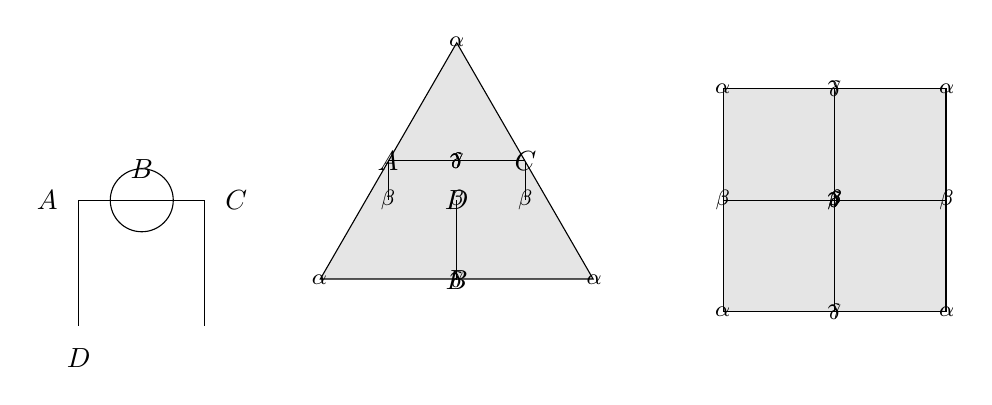
\begin{tikzpicture}[scale=0.8]
    % First diagram
    \draw (0,0) -- (2,0);
    \draw (1,0) circle (0.5);
    \draw (0,0) -- (0,-2);
    \draw (2,0) -- (2,-2);
    \node at (-0.5,0) {$A$};
    \node at (2.5,0) {$C$};
    \node at (0,-2.5) {$D$};
    \node at (1,0.5) {$B$};

    % Second diagram
    \begin{scope}[xshift=6cm]
        \node[regular polygon, regular polygon sides=3, minimum size=4cm, draw, fill=gray!20] (triangle) {};
        \foreach \i in {1,...,3} {
            \node at (triangle.corner \i) {\footnotesize $\alpha$};
        }
        \foreach \i in {1,2,3} {
            \draw (triangle.side \i) -- (triangle.side \i |- triangle.center);
            \node at (triangle.side \i |- triangle.center) {\footnotesize $\beta$};
        }
        \foreach \i in {1,2,3} {
            \draw (triangle.side \i) -- (triangle.side \i -| triangle.center);
            \node at (triangle.side \i -| triangle.center) {\footnotesize $\gamma$};
        }
        \node at (triangle.side 1 -| triangle.center) {\footnotesize $\delta$};
        \node at (triangle.side 2 -| triangle.center) {\footnotesize $\delta$};
        \node at (triangle.side 3 -| triangle.center) {\footnotesize $\delta$};
        \node at (triangle.center) {$D$};
        \node at (triangle.side 1) {$A$};
        \node at (triangle.side 2) {$B$};
        \node at (triangle.side 3) {$C$};
    \end{scope}

    % Third diagram
    \begin{scope}[xshift=12cm]
        \node[regular polygon, regular polygon sides=4, minimum size=4cm, draw, fill=gray!20] (square) {};
        \foreach \i in {1,...,4} {
            \node at (square.corner \i) {\footnotesize $\alpha$};
        }
        \foreach \i in {1,2,3,4} {
            \draw (square.side \i) -- (square.side \i |- square.center);
            \node at (square.side \i |- square.center) {\footnotesize $\beta$};
        }
        \foreach \i in {1,2,3,4} {
            \draw (square.side \i) -- (square.side \i -| square.center);
            \node at (square.side \i -| square.center) {\footnotesize $\gamma$};
        }
        \node at (square.side 1 -| square.center) {\footnotesize $\delta$};
        \node at (square.side 2 -| square.center) {\footnotesize $\delta$};
        \node at (square.side 3 -| square.center) {\footnotesize $\delta$};
        \node at (square.side 4 -| square.center) {\footnotesize $\delta$};
    \end{scope}
\end{tikzpicture}

\end{document}